\documentclass{beamer}
% 此处 type 无所谓
\usepackage{graphicx}
%\usepackage{ragged2e}
\usepackage{amsmath}
\usepackage{epstopdf}
%\usepackage{xeCJK}
%\setCJKmainfont{SimSun}
\begin{document}
%\begin{tabular}{p{7em}@{ }c}
%\hbox to 7em{姓 名:}&赵丰\\
%\hbox to 7em{指 导 老 师:}&沈渊\\
%\hbox to 7em{联合指导老师:}&梁恒
%\end{tabular}
%{
%\cleartabs
%{\+ \hbox to 7em{姓 名:}& 赵丰 \cr
%\+ \hbox to 7em{指 导 老 师:} & 沈渊\cr
%\+ \hbox to 7em{联合指导老师:}  & 梁恒\cr}
%\tabskip = 1em 
%\halign{%
%#\hfil&\hfil#\cr
%\hbox to 7em{姓 名:}& 赵丰\cr
%\hbox to 7em{指 导 老 师:} & 沈渊\cr
%\hbox to 7em{联合指导老师:}  & 梁恒\cr}
\begin{frame}
An abstract of a dissertation is a summary and extraction of research work
   and contributions. 
\begin{equation*}
T_1=\lambda+\cfrac{1}{1+\cfrac{\sin^2 \theta_1}{\lambda}+\cfrac{\cos^2\theta_1}{\lambda+\cfrac{1}{1+\cfrac{\sin^2 \theta_2}{\lambda}+\cfrac{\cos^2\theta_2}{\lambda+\boxed{\cfrac{1}{1+\cfrac{1}{\lambda}}}}}}}.
\end{equation*}
\vskip -6em
%\begin{tabular}{lc}
%$&\\
%\quad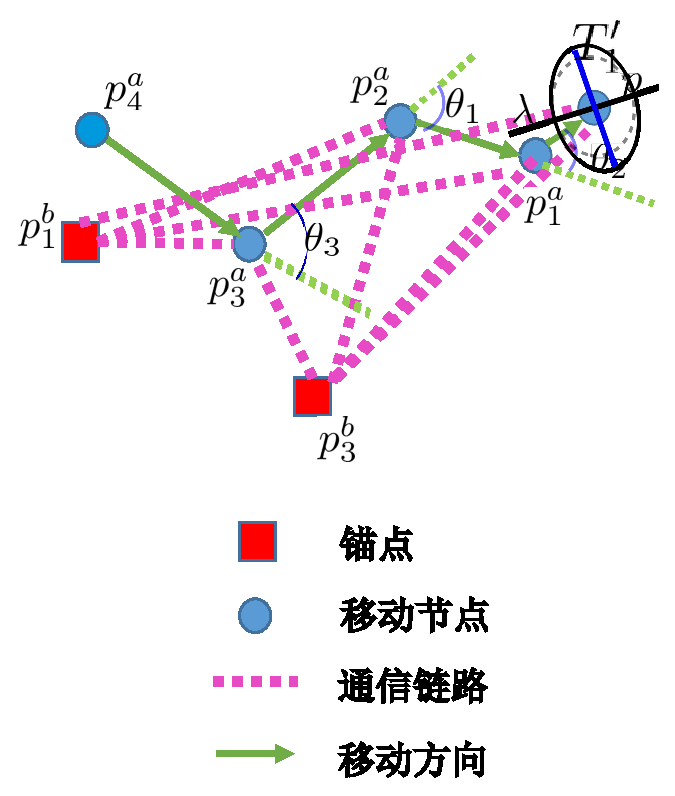
\includegraphics[width=120pt]{figures/cooperative_single_temporal_after.eps}%&\\
%\vskip -3em
%\raggedleft{
%\parbox[c][6em][t]{0.33\textwidth}{abstract of a dissertation is a summary and extraction of research work and contributions}
%}
%\parbox{abstract of a dissertation is a summary and extraction of research work and contributions}
%\end{tabular}
\end{frame}
\appendix
\begin{frame}
AppendixOne
\end{frame}
\begin{frame}
AppendixTwo
\end{frame}
\end{document}
